\documentclass[10pt,twocolumn,letterpaper]{article}

% ---------------------------------------------------------------
% Include basic CVPR package in rebuttal mode

\usepackage[rebuttal]{cvpr}

% ---------------------------------------------------------------
% Other packages

% Commonly used abbreviations (\eg, \ie, \etc, \cf, \etal, etc.)
\usepackage{eccvabbrv}
\setlength{\textfloatsep}{4pt plus 1pt minus 1pt}
\setlength{\intextsep}{4pt plus 1pt minus 1pt}
% Include other packages here, before hyperref.
\usepackage{graphicx}
\usepackage{booktabs}
\usepackage{pifont}
% The "axessiblity" package can be found at: https://ctan.org/pkg/axessibility?lang=en
\usepackage[accsupp]{axessibility}  % Improves PDF readability for those with disabilities.
\definecolor{dg}{rgb}{0,0.694,0.298}
\definecolor{purple}{rgb}{0.4,0.176,0.569}
\definecolor{royalblue}{RGB}{65,105,225}
\renewcommand{\thefigure}{\Alph{figure}}
\renewcommand{\thetable}{\Alph{table}}
% ---------------------------------------------------------------
% Hyperref package
% If you comment hyperref and then uncomment it, you should delete
% egpaper.aux before re-running latex.  (Or just hit 'q' on the first latex
% run, let it finish, and you should be clear).

\definecolor{eccvblue}{rgb}{0.12,0.49,0.85}
\usepackage[pagebackref,breaklinks,colorlinks,citecolor=eccvblue]{hyperref}


% ---------------------------------------------------------------
% If you wish to avoid re-using figure, table, and equation numbers from
% the main paper, please uncomment the following and change the numbers
% appropriately.
%\setcounter{figure}{2}
%\setcounter{table}{1}
%\setcounter{equation}{2}

% If you wish to avoid re-using reference numbers from the main paper,
% please uncomment the following and change the counter for `enumiv' to
% the number of references you have in the main paper (here, 6).
%\let\oldthebibliography=\thebibliography
%\let\oldendthebibliography=\endthebibliography
%\renewenvironment{thebibliography}[1]{%
%     \oldthebibliography{#1}%
%     \setcounter{enumiv}{6}%
%}{\oldendthebibliography}


% ---------------------------------------------------------------
% TODO REBUTTAL: Please enter paper ID
\def\paperID{*****} % *** Enter the paper ID here
\def\confName{ECCV}
\def\confYear{2026}

\begin{document}

% ---------------------------------------------------------------
% TODO REBUTTAL: Paper title is not required
%\title{\LaTeX\ Guidelines for Author Response}  % **** Enter the paper title here

%\maketitle
\thispagestyle{empty}
\appendix


% ---------------------------------------------------------------
% TODO REBUTTAL: Enter your response below
% We sincerely thank all reviewers for their constructive feedback.

\noindent\textbf{\textcolor{orange}{R1 (jnRs)}-Q1: Baseline.} Table~\ref{tab:Baseline} shows the I-frame-only baseline. Relying solely on I-frames is insufficient, validating the necessity of MV/Res fusion.
\vspace{-10pt}
\begin{table}[h]
\centering\tiny\resizebox{0.8\columnwidth}{!}{
\begin{tabular}{lccc}
\toprule
Modalities & Text Supervision & HMDB-51 & UCF-101 \\ \midrule
IF Only & w/o \textbf{Attribute} & 74.2 & 95.5 \\
IF Only & w/  \textbf{Attribute} & 73.4 & 95.4 \\
I + MV + Res & w/o \textbf{Attribute} & 74.4 & 95.1 \\ 
I + MV + Res(Ours) & w/  \textbf{Attribute} & \textbf{75.9} & \textbf{96.4} \\ \bottomrule
\end{tabular}}
\vspace{-8pt}
\caption{I-frame vs. compressed-domain modalities.}
\label{tab:Baseline}
\end{table}
\vspace{1pt}

\noindent\textbf{\textcolor{orange}{R1}-Q2: Semantic Specificity vs. Prompt Length.} We shuffled the attribute words across different categories using five random seeds and tested a dummy prompt: "This is a standard video clip showing a human performing an action in a specific environment with some motion and visual details." Table~\ref{tab:Correct_Attr} confirms gains come from \textbf{meaningful semantic matching}, not prompt length or introducing tokens.


\vspace{-1pt}
\begin{table}[h]
\centering\tiny\resizebox{0.8\columnwidth}{!}{
\begin{tabular}{lccc}
\toprule
Text Supervision & Semantic Match & HMDB-51 & UCF-101 \\ \midrule
Class Name Only & \ding{52} & 74.4 & 95.1 \\ 
Dummy Prompt & \ding{56} & 74.2 & 95.3 \\
Shuffled Attributes & \ding{56} & 74.2 & 95.5 \\
Correct Attributes(Ours) & \ding{52} & \textbf{75.9} & \textbf{96.4} \\ \bottomrule
\end{tabular}}
\vspace{-8pt}
\caption{Effect of semantic matching in attribute prompts.}
\label{tab:Correct_Attr}
\end{table}
\vspace{-4pt}

\noindent\textbf{\textcolor{orange}{R1}-Q3: Performance on SSv2.}  Limited absolute performance reflects coarse MV resolution, not a routing failure. Fig.~\ref{fig:iadf_weights} shows IADF significantly increases MV/Res weights on SSv2 over trainable fusion, confirming correct routing and directly boosting accuracy from 57.7\% to 60.4\%..

\vspace{-4pt}
\begin{figure}[h]
    \centering
    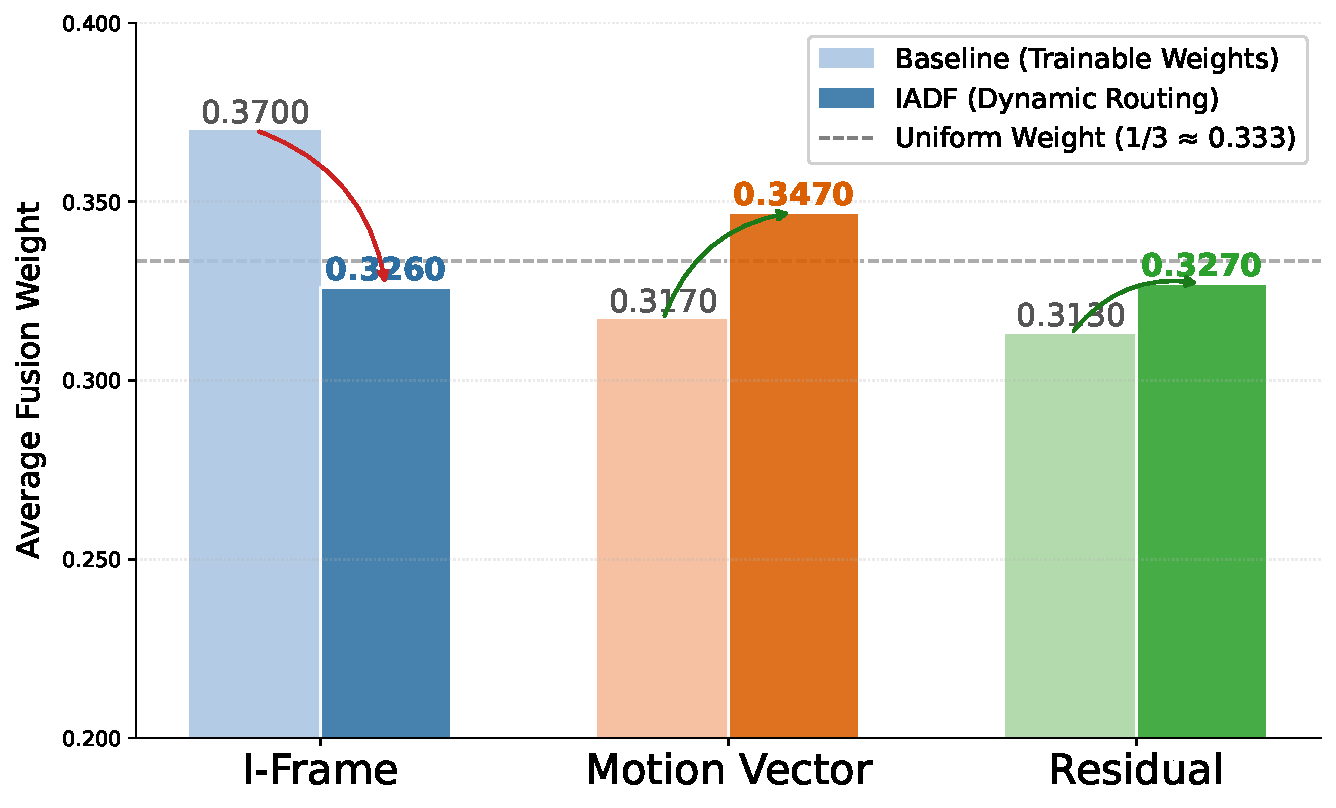
\includegraphics[width=0.7\linewidth]{fig1.pdf}
    \vspace{-10pt}
    \caption{Modality weights on SSv2 before/after IADF.}
    \label{fig:iadf_weights}
    \vspace{-6pt}
\end{figure}

\noindent\textbf{\textcolor{orange}{R1}-Q4: Novelty.}  We clarify the positioning. Compressed-domain signals (MV/Res) are semantically sparse and noisy, making direct text supervision ineffective—a gap absent in RGB methods. The novelty lies in identifying this problem and solving it: LLM attributes serve as a semantic bridge between text and heterogeneous compressed signals, enabling IADF's text-guided adaptive fusion and supporting zero/few-shot generalization without inference overhead.

\noindent\textbf{\textcolor{orange}{R1}-Q5: Typo.} Thanks for the review. Typo at L83 is fixed.

\noindent\textbf{\textcolor{blue}{R2(om4n)}-Q1: About Baseline.} We agree that the gain of each module is moderate. However, the full model improves from 74.4/95.2 to 76.2/96.7 on HMDB-51/UCF-101. IADF adds robustness under MV noise and stronger few/zero-shot gains. vs.\ HSINet-T (Guo et al., TCSVT 2026): +3.4/+0.0/+6.9 on HMDB-51/UCF-101/K400; vs.\ HSINet-B: +2.5 on K400 at lower cost; vs.\ CompViT (Wu et al., IJCV 2026)+K400PT: +0.9/+0.2/+1.8.

\noindent\textbf{\textcolor{blue}{R2}-Q2: Attribute Robustness and Inference Overhead.} Attributes are generated offline once, introducing zero inference overhead. To evaluate generation variance, regenerating 5 times yields 75.8$\pm$0.3\%, confirming stability. Prompt template sensitivity across 5 variants yields 76.0$\pm$0.4\%, indicating robustness to prompt design. On 10 HMDB-51 classes: baseline 73.2\%, manual 74.1\%, LLM 75.6\%, LLM candidates with manual selection 77.8\%, showing LLM attributes are strong and convenient.

\noindent\textbf{\textcolor{blue}{R2}-Q3: Fair Comparison.} We accept this critique and will revise all "state-of-the-art" claims to competitive compressed-domain performance. Comparing our model with CVPT-L and MM-ViT overlooks scale and computational gaps. At matched backbone scale, TextComp-L achieves 81.8\%/98.0\% on HMDB-51/UCF-101, surpassing CVPT ViT-L (81.5\%/98.0\%) without RGB decoding; the SSv2 gap reflects coarse MV resolution rather   than model failure, as detailed in R1-Q3.


\noindent\textbf{\textcolor{blue}{R2}-Q4: Motion vs. Appearance.} We analyzed class-level average IADF weights on HMDB-51. The dominant modality is I-frame for 22 classes, MV for 10 classes, and residuals for 19 classes, showing that IADF does not collapse to one modality. Motion-centric classes generally assign higher weights to motion-related compressed cues, i.e.MV+Res: throw 0.734, handstand 0.728, turn 0.723, and cartwheel 0.714. In contrast, appearance/posture/object-related classes show higher I-frame weights, e.g.shoot gun 0.406, sword 0.406, sit 0.403, and smoke 0.396.

\noindent\textbf{\textcolor{green!55!black}{R3(Bg4a)}-Q1: Novelty.} The novelty lies in solving the semantic gap unique to compressed video via LLM attributes, enabling zero/few-shot generalization absent in purely visual compressed-domain methods.

\noindent\textbf{\textcolor{green!55!black}{R3}-Q2: Fairness of Comparison.} As in \textbf{R2-Q3}, we revised overclaimed wording and added backbone-matched comparisons (ViT-L, HSINet, CompViT). Raw-video methods are included solely as an efficiency reference, not as SOTA claims within the compressed domain.

\noindent\textbf{\textcolor{green!55!black}{R3}-Q3: Attribute Quality.} We provide generation stability (75.8±0.3\% across 5 seeds), attribute quality comparisons (manual vs.\ LLM vs.\ LLM+manual selection), and sensitivity to attribute quantity $L$ (Sec.~4.6).

\noindent\textbf{\textcolor{green!55!black}{R3}-Q4: Text Baseline.} Using class name + IADF achieves 73.3\%/95.1\% on HMDB-51/UCF-101, while our attribute-enhanced version reaches 76.2\%/96.7\%, directly isolating the gain from attribute decomposition.

\noindent\textbf{\textcolor{green!55!black}{R3}-Q5: Text Branch vs.\ CLIP Init.} With compressed modalities and a classification head only (no text branch), K400-PT and CLIP-PT yield 62.9\% and 60.9\%. The full model reaches 76.2\%, confirming \textbf{+13.3\% comes from the text branch}, not CLIP initialization.

\noindent\textbf{\textcolor{green!55!black}{R3}-Q6: Failure Cases.} We observe two typical failure patterns. \textbf{Ambiguous Classes} (e.g. wave, stand) receive generic attributes, offering little gain over class-name baseline; \textbf{Similar Action Pairs} (e.g. pick vs.\ put) share overlapping attributes, causing misclassifications.


\end{document}
